\chapter{Systemarchitektur}
\begin{tiny}
MB
\end{tiny}
\section{Schichtenarchitektur}
	Um die Systemarchitektur von \glqq ofCourse\grqq{} besser zu veranschaulichen soll folgende Schichtenarchitektur dienen. Diese baut auf das Prinzip des Entwurfsmusters \glqq Model 2\grqq{} auf. \\ \\
    %Bild der Schichtenarchitektur
    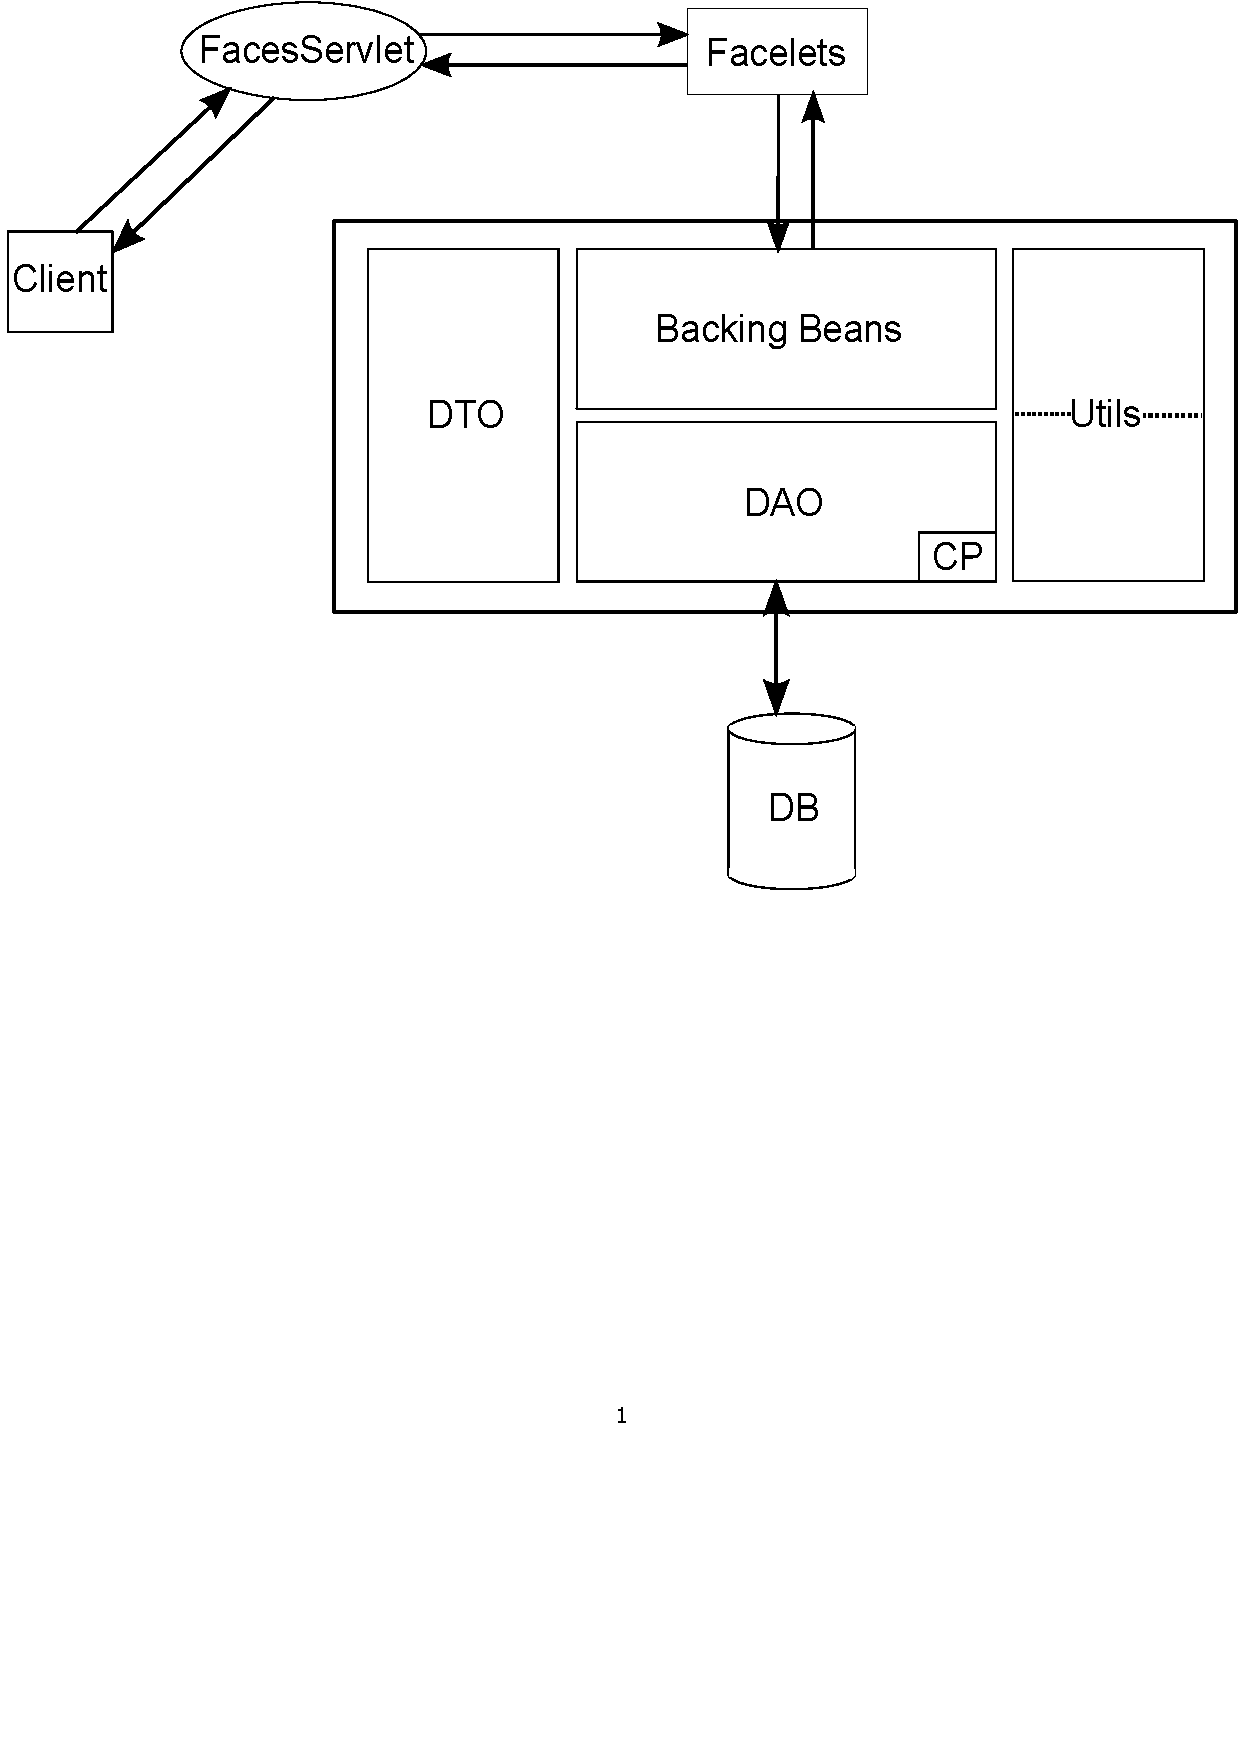
\includegraphics[scale=0.50]{Grafiken/Schichtenarchitektur.pdf}
	\subsection{Faces-Servlet}
	    Das Faces-Servlet fungiert im System als Controller, der eine HTTP-Request abfängt, diese bearbeitet, sowie weiterleitet. Das Faces-Servlet muss in jeder JSF-Applikation vorhanden sein und wird dementsprechend in der Webkonfigurationsdatei \textit{web.xml} definiert bzw. konfiguriert. 
    \subsection{Facelets}
    	Die View wird durch Facelets repräsentiert. Sie stellen die Inhalte dar, der vom Controller übergeben wird. Des Weiteren werden in der View die Benutzerinteraktionen entgegengenommen. Genauer auf Facelets wird unter Kapitel 4 Facelets eingegangen.
   	\subsection{Model}
   	Das Model kann in vier Bereiche unterteilt werden. Zunächst gäbe es die \glqq Upper Layer\grqq{}, welche die Backing Beans beinhalten, die \glqq Lower Layer\grqq{} mit den Data Access Objects (DAOs) und dem Connection Pool (CP), des Weiteren gäbe es noch die Data Transfer Objects (DTOs) und die Utils. 
   		\subsubsection{Upper Layer}
   		Die \glqq Upper Layer\grqq{} besteht aus den Backing Beans. In Diesen ist zum Einen die Geschäftslogik enthalten, zum Anderen werden dort die überlieferten Benutzereingaben der Facelets übergeben, weiterverarbeitet und gespeichert. Die Backing Beans werden in der zentralen JSF-Konfigurationsdatei \textit{faces-config.xml} verwaltet.
    	\subsubsection{Lower Layer}
    	In der \glqq Lower Layer\grqq{} befinden sich die Data Access Objects und der Connection Pool. Mithilfe der im CP lagernden Datenbankverbindungen greifen die DAOs auf die darunterliegende Database (DB) zu.
    	\subsubsection{DTO}
    	Die Data Transfer Objects dienen als Schnittstelle zwischen den Backing Beans und den zugehörigen DAOs. Sie bündeln logisch zusammenhängende Daten in einem Objekt, um zeitintensive Fernzugriffe durch einen zu ersetzen.
    	\subsubsection{Utils}
    	Utils fungieren als Hilfs- und Verwalterklasse. Die Utils werden auch wiederum unterteilt, die man entweder den Backing Beans oder den DAOs zuordnen kann. 
    \subsection{Database}
    Für die persistente Speicherung von Daten ist die Database (DB) zuständig. Dort werden Daten wie z.B. \textit{BenutzerID, Benutzername, Kurseinheit, Kurslehrer} etc. gespeichert. Zugriff auf die DB haben nur die DAOs. 

\section{Package-Diagramm}
 Um einen kleinen Überblick der verwendeten Packages im System zu bekommen, soll die folgende Figur dazu Abhilfe schaffen. \\ 
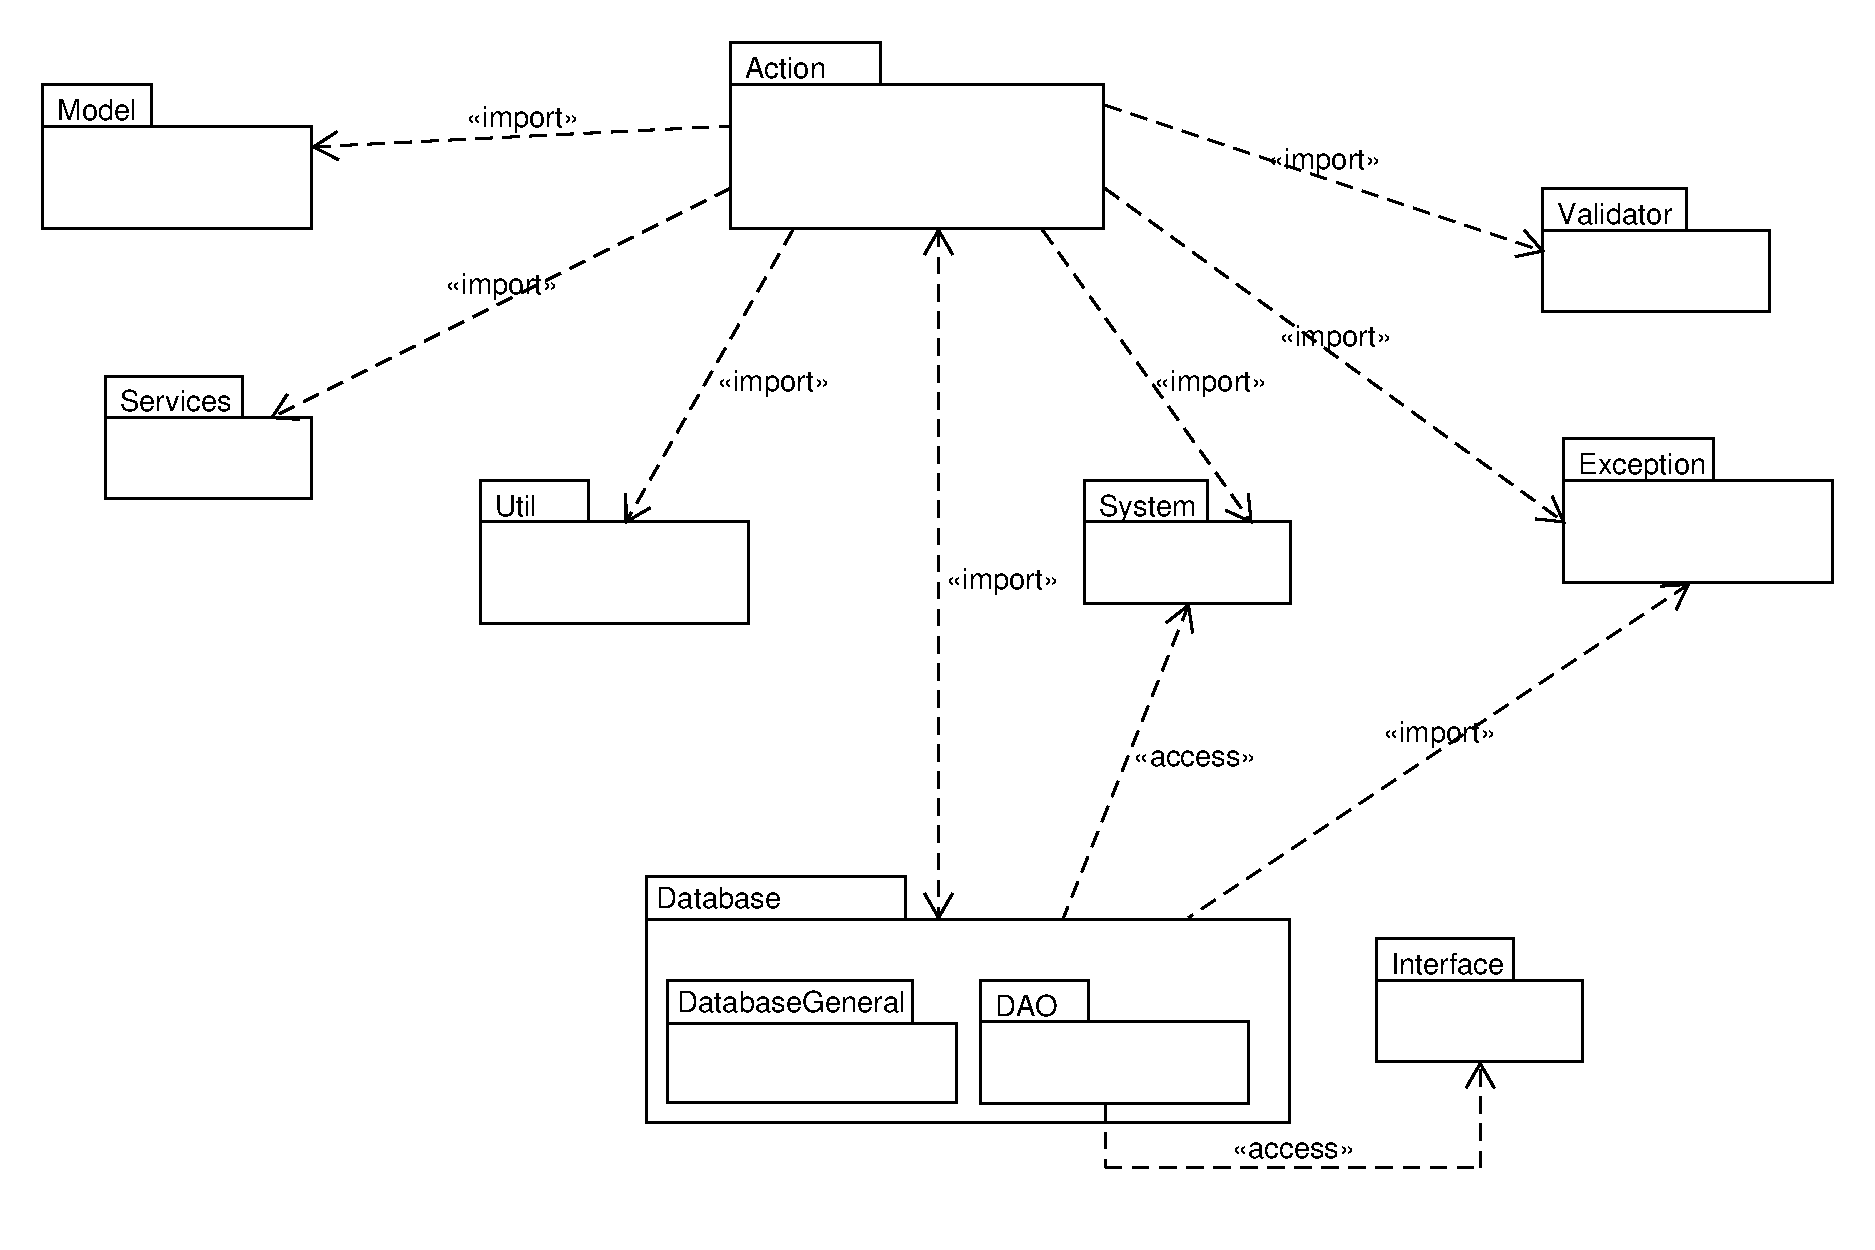
\includegraphics[scale=0.45]{Grafiken/PackageDiagramm.pdf}      
    
\section{Design Patterns}
Damit keine wiederkehrenden Entwurfsprobleme bei der Softwareentwicklung auftreten, werden bewährte Lösungsansätze, die sogenannten \glqq Design Patterns\grqq{}, benutzt. Sie dienen dazu den Entwurf möglichst flexibel, erweiterbar und auch einfach zu gestalten. Aufgrund dessen werden im Nachfolgendem die für das System eingesetzten \textit{Design Patterns} beschrieben:
	\begin{itemize}
		\item \textbf{Model 2:} Bei dem Architekturmuster \textit{Model 2} wird die View (Facelets) von der Geschäftslogik (Backing Beans) bei einer Java-Webapplikation getrennt. Der Ablauf sieht im Groben so aus, dass ein HTTP-Request eines Clients an den Controller (Faces-Servlet) weitergeleitet wird. Darauffolgend \glqq steuert\grqq{} der Controller alle notwendigen Schritte zur Beschaffung des Inhalts für die Darstellung. Der Controller legt den Inhalt in einer Backing Beans ab und entscheidet, welcher View der Inhalt übergeben wird. Die View wiederum stellt den Inhalt dar, der vom Controller weitergereicht wurde.
		\item \textbf{Data Transfer Object:} Das DTO fasst mehrere Daten in einem Objekt zusammen, damit sie in einem Aufruf übergeben werden. Somit können Datensätze durch die Schichten transportiert werden.
		\item \textbf{Dependency Injection:} Dependency Injection ist ein JSF Standard, um Backing Beans zu verwalten. Hierbei werden die benötigten Objekte an einem zentralen Ort hinterlegt, was auch die Flexibilität erhöht.  
		\item \textbf{Creational Pattern:} Die Creational Patterns sind eine Teilmenge der Design Patterns und dienen als Entwurfsmuster für die Erzeugung von Objekten. Man kann diese in folgende Pattern unterscheiden.
			\begin{itemize}
				\item \textbf{Factory Pattern:} Bei diesem Pattern werden mehrere ähnliche Objekte durch Aufruf einer Methode anstatt durch direkten Aufruf eines Konstruktors erzeugt.
				\item \textbf{Object Pooling:} Beim Object Pooling werden ressourcenintensive Objekte (hier Datenbankverbindungen) in einem Pool (Connection Pool) bereitgehalten, um sie bei Bedarf erneut nutzen zu können, was sich wiederum positiv auf die Ausführungszeit auswirkt.
				\item \textbf{Singleton:} Es soll sichergestellt werden, dass von einem Objekt jeweils nur eine Instanz existiert. Diese sind darüber hinaus global verfügbar.  
			\end{itemize}
	\end{itemize}
\section{Einsatz externer Libraries}
Es werden im System auf bereits vorhandenen Libraries zurückgegriffen.
	\begin{itemize}
		\item \textbf{PostgreSQL JDBC 9.4-1201:} Der PostgreSQL JDBC-Treiber wird für die Kommunikation mit der Datenbank verwendet.
		\item \textbf{JSF 2.2:} Für die Implementierung von JSF wird das Framework Mojarra 2.2.10 benutzt.
		\item \textbf{JavaMail API 1.5.2:} Library für das Versenden von Emails.
		\item \textbf{Bootstrap 3.3.0:} Bootstrap dient als Grundlage für das Design der Facelets.
		\item \textbf{Tomcat 8.0.21:} Webcontainer, um die in Java geschriebenen Webapplikationen auszuführen.
		\item \textbf{Log4J:} Library für das Loggen von Meldungen.
	\end{itemize}
\section{Fehlerbehandlung}
	\subsection{Nicht-Autorisierter Zugriff}
	Sofern der User eine Aktion ausführen will, aber nicht die entsprechenden dafür Rechte besitzt, wird eine Fehlermeldung ausgegeben. Beispielsweise will sich ein Gast bestimmte Details eines Kurs ansehen, was aber nur registrierte User vorbehalten ist. Dem Gast wird eine Fehlermeldung angezeigt und gegebenenfalls auf die Login Seite verwiesen. Zur Realisierung hierfür werden die Facelets von einem Phaselistener überprüft.
	\subsection{Fehlerhafte Benutzereingaben}
	Wenn ein Gast sich registrieren will, aber in den Formulardaten eine ungültige Eingabe tätigt, so soll der Gast nicht alles neu eingeben müssen, sondern nur die fehlerhaften Stellen neu. Der Fehler wird auf derselben Seite angezeigt, somit wird keine Fehler-Seite extra benötigt.
	\subsection{Exceptions}
	Sollten Fehler auftreten auf die der User keinen Einfluss hat, so wird der Nutzer auf eine Fehler-Seite geleitet. Auf dieser Seite befinden sich Informationen zu dem Fehler und es wird eine weitere Vorgehensweise zur Verfügung gestellt. Bestimmte Exceptions wie beispielsweise eine SQL-Exception werden gefangen und geworfen, indem globale Exception-Handler implementiert werden. Bei kritischen Exceptions wird auch eine Logfile angefertigt, um im Nachhinein genau zu verfolgen wo und wann der Fehler aufgetreten ist.
	\subsection{HTTP-Statuscodes}
	Für den User werden HTTP-Statuscodes generiert. Somit bleiben kryptische Fehlermeldungen seitens des Webservers dem User verborgen. Dem User werden die Fehler auf einer neuen Seite angezeigt: \\ \\
	\begin{tabular}{|l|l|}
		\hline
		Status Code & Beschreibung \\
		\hline
		403 & Zugriff nicht autorisiert \\
		404 & Datei/Ressource nicht vorhanden \\
		408 & Server-Timeout \\
		500 & Interner Server Fehler \\
		503 & Server nicht erreichbar \\
		\hline
 	\end{tabular}		     

